\documentclass{journalstyle}




\title{Tests for an Increasing Trend in the Intensity of a Poisson Process: A Power Study}
\author{Maxime Baba, Mathile Ferreira, Félix Foucher de Brandois}
\newcommand{\footertext}{ModIA - INSA / ENSEEIHT, \\ 2024-2025}

\begin{document}


\maketitle

%\tableofcontents
%\listoffigures



%\section*{Introduction}

A Nonhomogeneous Poisson Process (NHPP) is a stochastic process often used to model phenomena where the rate of occurrence of events changes over time.
The rate, or intensity function $\lambda(t)$, represents the expected number of events per unit time at a given time $t$.
Understanding and analyzing the behavior of this rate is crucial in diverse fields such as reliability engineering, healthcare, and environmental studies, as it helps identify patterns, predict future events, and optimize interventions.
Detecting increasing trends in the rate can be particularly important, for example, in monitoring system deterioration or identifying escalating risks in processes.
Although various statistical methods have been proposed to identify increasing trends in NHPPs, existing treatments—such as those by Bain, Engelhardt, and Wright \cite{BainEngelhardtWright}—lack clarity and precision in both theoretical explanation and practical application.
Our study addresses these shortcomings by providing a detailed exploration of the Laplace test and Boswell’s likelihood ratio test.
The paper is structured in three parts: a theoretical discussion of the selected tests, numerical simulations comparing their performance, and an application to real-world data.


\section{Theoretical Framework for Trend Detection Tests}

A statistical test evaluates two competing hypotheses: the null hypothesis $H_0$ (representing the status quo) and the alternative hypothesis $H_1$ (indicating a deviation from $H_0$).
Based on the sample data, a test statistic is computed and compared to a critical threshold.
If the test statistic exceeds this threshold, $H_0$ is rejected in favor of $H_1$. \\
In our case, we test whether the intensity function $\lambda(t)$ of a Poisson process is constant ($H_0$) or increasing ($H_1$).

\subsection{Laplace Test}

Let $(N(t))_{t \geq 0}$ be a Poisson process with intensity function $\lambda(t)$.
We observe $N(t)$ in the interval $[0, T^*]$.
Let $0 < T_1 < T_2 < \ldots < T_n < T^*$ be the ordered observation times. \\

\noindent\textbf{Test Statistic} \\
Under $H_0$, the arrival times $T_1, \ldots, T_n$ (conditioned on $N_{T^*} = n$) behave like order statistics from a uniform distribution.
Specifically: \\
$(T_1, \ldots, T_n) | \{N_{T^*} = n\} \overset{(d)}{=} (U_1, \ldots, U_n)$, where $U_1, \ldots, U_n \underset{i.i.d.}{\sim} \mathcal{U}([0, T^*])$. \\
Therefore, $(\frac{T_1}{T^*}, \ldots, \frac{T_n}{T^*}) | \{N_{T^*} = n\} \overset{(d)}{=} (V_1, \ldots, V_n)$, where $V_1, \ldots, V_n \underset{i.i.d.}{\sim} \mathcal{U}([0, 1])$. \\
Define the Laplace test statistic as: 
\begin{equation}
    F = \frac{1}{T^*} \sum_{i=1}^n T_i.
    \label{eq:laplace_test_statistic}
\end{equation}

By the Central Limit Theorem, under $H_0$,  can be standardized as: 
$Z = \frac{F - \mathbb{E}[F]}{\sqrt{\text{Var}(F)}} = \frac{F - \frac{n}{2}}{\sqrt{\frac{n}{12}}} \sim \mathcal{N}(0, 1)$
for large $n$. \\

\noindent\textbf{Decision Rule} \\
If the intensity $\lambda(t)$ is increasing, the arrival times $T_i$ are expected to cluster towards the end of the interval $[0, T^*]$, making $F$ larger.
Therefore, we reject $H_0$ if $F \geq s_{\alpha}$, where $s_{\alpha}$ is the critical threshold determined as: $s_{\alpha} = \frac{n}{2} + z_{1 - \alpha} \sqrt{\frac{n}{12}}$. \\
with $z_{1 - \alpha}$ being the $(1 - \alpha)$-th quantile of the standard normal distribution. \\

\noindent\textbf{P-value} \\
The p-value measures the probability of obtaining a test statistic at least as extreme as the observed $F_{\text{obs}}$, under $H_0$.
It is given by:
\begin{equation}
    \hat{\alpha} = \mathbb{P}_{H_0}(F \geq F_{\text{obs}}) = 1 - \Phi\left(\frac{F_{\text{obs}} - \frac{n}{2}}{\sqrt{\frac{n}{12}}}\right)
    \label{eq:laplace_p_value}
\end{equation}

\noindent\textbf{Power} \\
The power of the test is the probability of rejecting $H_0$ when $H_1$ is true. \\
$\pi(\lambda) = \mathbb{P}_{H_1}(F \geq s_{\alpha})$.


\subsection{Boswell's Likelihood Ratio Test}

The goal of Boswell's test is to maximize the likelihood function under the constraint that the intensity function $\lambda(t)$ is non-decreasing.
Since the likelihood function involves the intensity values at the observed failure times, we look for the optimal estimates $\hat{\lambda}(T_i)$ that satisfy this constraint. \\

Let $(N(t))_{t \geq 0}$ be a Poisson process with intensity function $\lambda(t)$.
Consider the number $N_{T^*}$ of "events" that have occurred in $[0, T^*]$, and denote $T_1, \ldots, T_{N_{T^*}} < T^*$ the corresponding arrival times. \\


\noindent\textbf{Likelihood Function Recap} \\
The likelihood function for the observation times $T_1, \ldots, T_n$, conditioned on $N_{T^*} = n$, is given by:
$$
\mathcal{L}((T_i)_{1 \leq i \leq n}; \lambda) = \left(\prod_{i=1}^n \lambda(T_i)\right) \exp\left(-\int_0^{T^*} \lambda(t) dt\right)
$$

We assume that the intensity function $\lambda(t)$ is piecewise constant and non-decreasing between successive failure times $T_{i}$ and $T_{i+1}$.
Therefore, we need to determine the values $\hat{\lambda}(T_i)$ that maximize this likelihood. \\

\noindent\textbf{Formulating the Optimization Problem} \\
Under the previous assumptions (with $T_{n+1} = T^*$): \\
$\int_0^{T^*} \lambda(t) dt = \sum_{i=1}^n (T_{i+1} - T_i) \lambda(T_i)$ \\

\noindent We want to find $\hat{\lambda}(T_i)$ that maximizes: \\
$\prod_{i=1}^{n} \lambda(T_i) \exp(-(T_{i+1} - T_i) \lambda(T_i))$ \\

This can be rewritten as: \\
\begin{equation*}
    \begin{split}
        &\underset{\lambda}{\text{max}} \prod_{i=1}^{n} f_i(\lambda(T_i)) \\
        \text{where } &f_i(x) = x \exp(-(T_{i+1} - T_i) x)
    \end{split}
    \label{eq:boswell_optimization_problem}
\end{equation*}

The function $f_i(x)$ is unimodal, meaning it has a unique maximum.
According to Boswell's theorem \cite{Boswell1966}, following the works of Brunk and von Eeden \cite{VanEeden1956}, the likelihood is maximized by the non-decreasing function $\hat{\lambda}(t)$ given by: \\
\begin{equation*}
    \begin{split}
        &\hat{\lambda}(T_i) = \underset{1 \leq \alpha \leq i}{\text{max}} \underset{i \leq \beta \leq n}{\text{min}} M(\alpha, \beta) \\
        \text{where } &M(\alpha, \beta) \text{ is the maximum of } x \mapsto \prod_{i=\alpha}^{\beta} f_i(x)
    \end{split}
    \label{eq:boswell_optimal_lambda}
\end{equation*}

We can find the form of $M(\alpha, \beta)$ by derviating the product of $f_i(x)$ and setting it to zero. \\
This leads to: \\
\begin{equation}
    \hat{\lambda}(T_i) = \underset{1 \leq \alpha \leq i}{\text{max}} \underset{i \leq \beta \leq n}{\text{min}} \frac{\beta - \alpha + 1}{T_{\beta + 1} - T_{\alpha}}
    \label{eq:boswell_optimal_lambda_formula}
\end{equation}

\noindent\textbf{Test Statistic} \\
The likelihood ratio test (LRT) compares the likelihood of the data under the null hypothesis $H_0$ (constant intensity) with the likelihood under the alternative hypothesis $H_1$ (non-decreasing intensity).
The test statistic is defined as: \\
$$
W = -2 \log \left( \frac{\text{sup }_{\lambda \in \Lambda_0} \mathcal{L}(\lambda)}{\text{sup }_{\lambda \in \Lambda} \mathcal{L}(\lambda)} \right)
$$
where $\Lambda_0$ is the set of constant intensity functions and $\Lambda$ is the set of non-decreasing intensity functions. \\

Under $H_0$, the maximum likelihood estimate of $\lambda(t)$ is $\lambda_0(t) = \frac{N_{T^*}}{T^*} = \frac{n}{T^*}$. \\
The log-likelihood under $H_0$ is:
$$
\log\mathcal{L}(\lambda_0) = \sum_{i=1}^n \log(\lambda_0(T_i)) - T^* \lambda_0 = n \log\left(\frac{n}{T^*}\right) - n
$$

Under $H_1$, the maximum likelihood using the optimal estimate $\hat{\lambda}(t)$ is:
$$
\log\mathcal{L}(\hat{\lambda}) = \sum_{i=1}^n \log(\hat{\lambda}(T_i)) - \int_0^{T^*} \hat{\lambda}(t) dt
$$
By Grenander's lemma \cite{Grenander1956}, we know that: \\
$\int_0^{T^*} \hat{\lambda}(t) dt = n$ \\

Therefore, the test statistic $W$ becomes (results are detailed in the appendix):
\begin{equation}
    W = 2 \left( \sum_{i=1}^{n} \log(\hat{\lambda}(T_i)) + n \log\left(\frac{T^*}{n}\right) \right)
    \label{eq:boswell_test_statistic}
\end{equation}

According to Wilks' theorem \cite{Wilks1938}, the distribution of the test statistic $W$ asymptotically approaches a $\chi^2$ distribution under the null hypothesis $H_0$.
The degrees of freedom of this distribution are equal to the difference in dimensionality between $\Lambda$ and $\Lambda_0$. \\

We assumed the intensity function $\lambda(t)$ is non-decreasing and can potentially exhibit multiple change points.
Suppose there are $k$ change points, this implies there are $k + 1$ regions where the intensity remains constant.
The possible ways that the $n$ observed failure times can be grouped into $k$ segments are given by the Stirling numbers of the first kind $s(n, k)$ \cite{StirlingNumbers}. \\
We can therefore compute the survival function of the test statistic $W$ under $H_0$ by summing the probabilities of the $\chi^2(k+1)$ distribution for all possible numbers of segments $k$, weighted by the probability of having $k$ segments.
\begin{equation}
    \mathbb{P}_{H_0}(W \geq w) \approx \sum_{k=1}^{n} \frac{s(n, k)}{n!} \mathbb{P}(\chi^2(k+1) \geq w)
    \label{eq:boswell_survival_function}
\end{equation}


\noindent\textbf{Decision Rule} \\
The decision rule for the LRT is based on the critical threshold $w_{\alpha}$. 
If $W \geq w_{\alpha}$, we reject $H_0$. $w_{\alpha}$ is determined as the $(1 - \alpha)$-th quantile of the previous distribution \eqref{eq:boswell_survival_function}. \\

\noindent\textbf{P-value} \\
The p-value is the probability of obtaining a test statistic at least as extreme as the observed $W_{\text{obs}}$ under $H_0$. 
It is given by: \\
$\hat{\alpha} = \mathbb{P}_{H_0}(W \geq W_{\text{obs}})$. \\

\noindent\textbf{Power} \\
The power of the test is the probability of rejecting $H_0$ when $H_1$ is true: \\
$\pi(\lambda) = \mathbb{P}_{H_1}(W \geq w_{\alpha})$. \\




\section{Numerical Simulations}

\subsection{Simulation Methodology}

We simulate data from a Nonhomogeneous Poisson Process (NHPP) with various intensity functions $\lambda(t)$:
\begin{itemize}
    \item Exponential trend: $\lambda(t) = e^{\beta t}$, with $\beta \geq 0$
    \item Weibull trend: $\lambda(t) = \beta t^{\beta - 1}$, with $\beta \geq 1$
\end{itemize}

We generate the arrival times $T_1, \ldots, T_n \in [0, T^*]$ using the inverse transform method.
Then, we perform a Monte Carlo simulation to compare the power of the Laplace test and Boswell's test under different conditions (e.g., intensity function shape, time interval $T^*$). \\
In order to be consistent with the results of the article studied \cite{BainEngelhardtWright}, we fix $T^*$ and $n$ at the same time, with the aim of reproducing similar results. \\

\noindent\textbf{Monte Carlo Simulation Principle} \\
\begin{enumerate}
    \item For each scenario, generate $N$ independent datasets.
    \item For each dataset, apply both the Laplace test and Boswell's likelihood ratio test and record whether the null hypothesis $H_0$ is rejected.
    \item The power $\pi$ of each test is estimated as the proportion of datasets where $H_0$ is rejected: $\pi = \frac{\text{Number of rejections of } H_0}{N}$.
\end{enumerate}

Boswell and Brunk \cite{Boswell1966} observed empirically that the large sample approximation for the LRT yields a true significance level somewhat larger than the nominal level.
We verified this observation in our simulations using Monte Carlo simulations.
Therefore, we adjusted the critical threshold for the LRT in our simulations to ensure the true significance level matches the nominal level.

\newpage

\subsection{Power Analysis}



\subsubsection{Exponential Trend}

The power of the Laplace and Boswell tests is calculated for different values of $T^*$. \\
The figure \ref{fig:power_exponential_beta} shows the power curves of the two tests in function of $\beta$. \\
\begin{figure}[H]
    \centering
    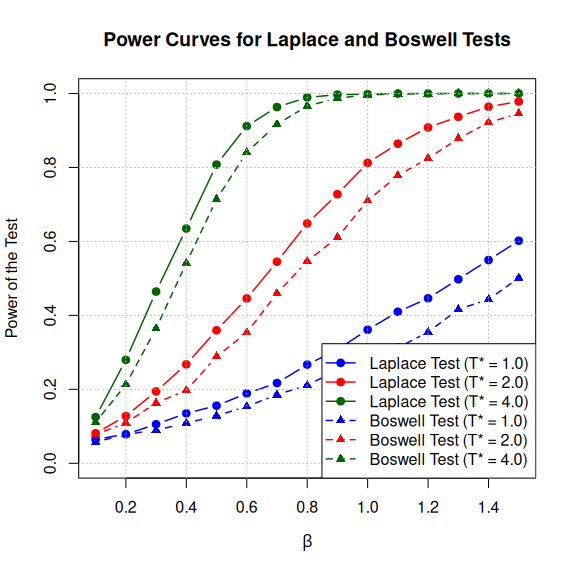
\includegraphics[width=0.4\textwidth]{src/power_exponential.png}
    \caption{Power Curves for Exponential Trend}
    \label{fig:power_exponential_beta}
\end{figure}

As $T^*$ increases (from $1.0$ to $4.0$), the power of both tests increases significantly.
This suggests that larger $T^*$ values improve the ability of both the Laplace and Boswell tests to detect deviations from the null hypothesis.
The Laplace test (solid lines with circle markers) consistently shows higher power compared to the Boswell test (dashed lines with triangle markers) for the same $T^*$ and $\beta$. \\


\subsubsection{Weibull Trend}

The power of the Laplace and Boswell tests is calculated for different values of $T^*$. \\
We observed that the power of the both tests does not vary significantly with the time interval $T^*$.
Therefore, we present the power curves for a fixed $T^*$.
The figure \ref{fig:power_weibull_beta} shows the power curves of the two tests in function of $\beta$. \\
\begin{figure}[H]
    \centering
    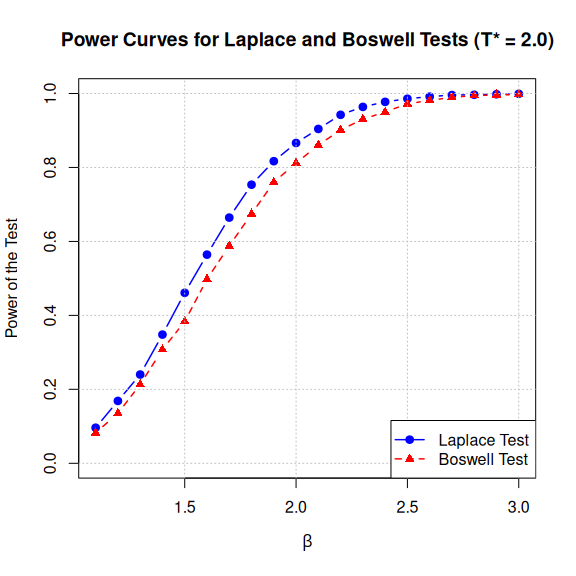
\includegraphics[width=0.4\textwidth]{src/power_weibull.png}
    \caption{Power Curves for Weibull Trend}
    \label{fig:power_weibull_beta}
\end{figure}


Once again, we are dealing with an increasing intensity.
Since Weibull intensity increases less rapidly than exponential trending, we see that exponential intensity takes less time to reach a higher power.
The Laplace test is still more powerful than the Boswell test, but the difference is less pronounced than for the exponential intensity. \\


\section{Application to Real-World Data}

We applied the Laplace test and Boswell's likelihood ratio test to a real-world dataset to detect an increasing trend in the intensity of a Poisson process.

\subsection{Description of the Dataset}

The dataset contains large fire insurance claims in Denmark from 1980 to 1990.
We are primarily interested in the arrival times of the claims to determine if there is an increasing trend in the intensity of claims over time. \\
The figure \ref{fig:fire_insurance_claims} shows the distribution of the arrival times of the claims.
Given the large number of claims ($n = 2166$), if the intensity of claims were constant, we would expect the curve to be relatively flat along the diagonal. \\

\begin{figure}[H]
    \centering
    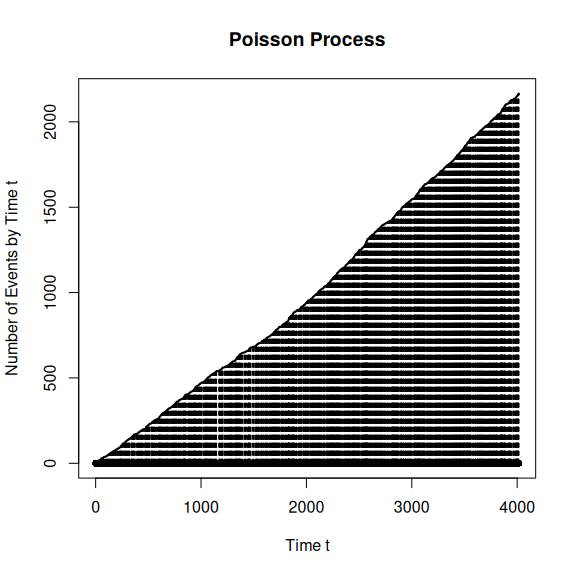
\includegraphics[width=0.4\textwidth]{src/fire_insurance_claims.png}
    \caption{Arrival Times of Fire Insurance Claims}
    \label{fig:fire_insurance_claims}
\end{figure}

The curve shows a slight upward trend, suggesting that the intensity of claims may be increasing.

\subsection{Dataset Analysis}

To justify the use of the Laplace and Boswell tests, we must ensure the process satisfies some assumptions of a Poisson process (exponential distribution and independence). \\

Figure \ref{fig:exponential_fit} shows the fit of an exponential distribution to the observed intervals. \\

\begin{figure}[H]
    \centering
    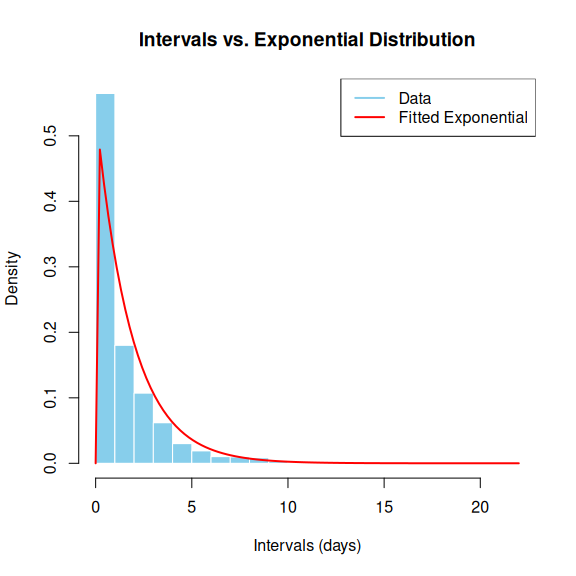
\includegraphics[width=0.4\textwidth]{src/exponential_fit.png}
    \caption{Exponential Fit to Time Intervals}
    \label{fig:exponential_fit}
\end{figure}

The fitted curve aligns reasonably well with the observed data, suggesting that the intervals between claims approximate an exponential distribution.
However, this fit alone does not confirm the process is homogeneous (i.e., with a constant rate). \\

We then need to check if the time intervals are independent.
The figure \ref{fig:correlation_intervals} shows the correlation between each interval.

\begin{figure}[H]
    \centering
    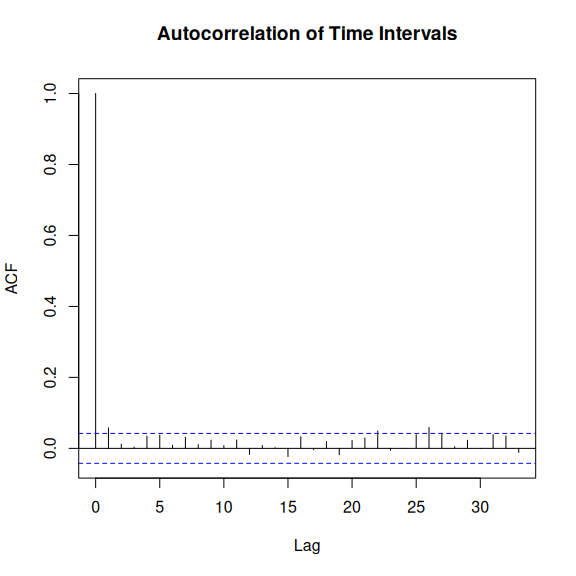
\includegraphics[width=0.4\textwidth]{src/correlation_intervals.png}
    \caption{Correlation between Time Intervals}
    \label{fig:correlation_intervals}
\end{figure}

The correlations between intervals tend to zero, indicating that the time intervals are independent.
This supports the assumption that the data can be modeled as a Poisson process.


\subsection{Applying the Tests}
We applied the Laplace test and Boswell's likelihood ratio test to the fire insurance claims dataset to detect an increasing trend in the intensity of claims over time. \\

\noindent\textbf{Laplace Test} \\
The Laplace test statistic $F$ was calculated using the formula \eqref{eq:laplace_test_statistic}.
We then used the p-value formula \eqref{eq:laplace_p_value} to compute the p-value, and obtained a value of approximately $10^{-4}$.
Since this p-value is below the significance level of $0.05$, we reject the null hypothesis that the intensity is constant. \\

\noindent\textbf{Boswell's Likelihood Ratio Test} \\
The Boswell test statistic $W$ was calculated using the formula \eqref{eq:boswell_test_statistic}.
However, we were unable to correctly implement the p-value for the Boswell test, as it requires to compute Stirling numbers of the first kind and a factorial of a large number, which is computationally expensive.
We tried to bypass this issue by using a logaritmic transformation, but the results were not satisfactory. \\
We also tried to find an asymptotic approximation of the threshold $w_{\alpha}$ to compare the test statistic $W$ to: \\

\begin{figure}[H]
    \centering
    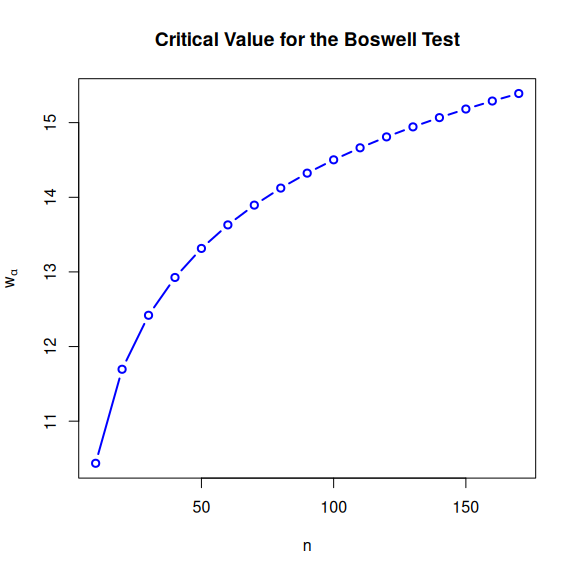
\includegraphics[width=0.4\textwidth]{src/walpha_approximation.png}
    \caption{Approximation of the Threshold $w_{\alpha}$}
    \label{fig:walpha_approximation}
\end{figure}

The figure \ref{fig:walpha_approximation} shows the value of the threshold $w_{\alpha}$ for different values of $n$ (with $\alpha = 0.04$). \\
We can see that the threshold don't seems to converge to a fixed value, as it keeps increasing with $n$.
We can't therefore predict its value for our dataset.


\section{Conclusion}
The primary aim of this report was to evaluate the performance of the Laplace test and Boswell's likelihood ratio test in detecting increasing trends in the intensity of a Nonhomogeneous Poisson Process (NHPP).
Using simulated data generated under exponential and Weibull intensity functions, as well as real-world fire insurance claims data, we compared the power of these two statistical tests under various conditions. \\
Our results show that the Laplace test consistently outperforms Boswell's test in detecting increasing trends in the intensity of a Poisson process.
When applying these tests to real-world fire insurance claims data, the Laplace test identified a statistically significant increasing trend in claim intensity, while the Boswell test could not be fully implemented due to computational limitations. \\
Future studies could explore computational improvements for Boswell's test to overcome its limitations and allow for more reliable comparisons.
Additionally, further research could investigate the performance of these tests under different types of intensity functions, such as cyclic or piecewise trends.


\printbibliography

\newpage
\end{multicols}

\appendix

\section{Boswell's Likelihood Ratio Test: Survival Function Calculation}

The likelihood function for the observation times $T_1, \ldots, T_n$, conditioned on $N_{T^*} = n$, is given by:
$$
\mathcal{L}((T_i)_{1 \leq i \leq n}; \lambda) = \left(\prod_{i=1}^n \lambda(T_i)\right) \exp\left(-\int_0^{T^*} \lambda(t) dt\right)
$$

We assume that the intensity function $\lambda(t)$ is piecewise constant and non-decreasing between successive failure times $T_{i}$ and $T_{i+1}$:
\begin{equation*}
    \begin{split}
        &\int_0^{T^*} \lambda(t) dt = \sum_{i=1}^n (T_{i+1} - T_i) \lambda(T_i) \\
        &\Leftrightarrow \left(\prod_{i=1}^n \lambda(T_i)\right) \exp\left(-\sum_{i=1}^n (T_{i+1} - T_i) \lambda(T_i)\right) \\
        &\qquad = \prod_{i=1}^n \lambda(T_i) \exp(-(T_{i+1} - T_i) \lambda(T_i)) \\
        &\qquad = \prod_{i=1}^n f_i(\lambda(T_i)) \\
        &\text{where } f_i(x) = x \exp(-(T_{i+1} - T_i) x)
        \end{split}
\end{equation*}

We prove that the functions $f_i(x)$ are unimodal:
\begin{equation*}
    \begin{split}
        &f_i'(x) = (1 - (T_{i+1} - T_i) x) \exp(-(T_{i+1} - T_i) x) \\
        &\begin{cases}
            f_i'(x) > 0 & \text{if } x < \frac{1}{T_{i+1} - T_i} \\
            f_i'(x) < 0 & \text{if } x > \frac{1}{T_{i+1} - T_i}
        \end{cases}
    \end{split}
\end{equation*}

Therefore, the function $f_i(x)$ has a unique maximum at $x = \frac{1}{T_{i+1} - T_i}$.

According to Boswell's theorem, the likelihood is maximized by the non-decreasing function $\hat{\lambda}(t)$ given by:
\begin{equation*}
    \begin{split}
        &\hat{\lambda}(T_i) = \underset{1 \leq \alpha \leq i}{\text{max}} \underset{i \leq \beta \leq n}{\text{min}} M(\alpha, \beta) \\
        &\text{where } M(\alpha, \beta) \text{ is the maximum of } x \mapsto \prod_{i=\alpha}^{\beta} f_i(x)
    \end{split}
\end{equation*}

We can find the form of $M(\alpha, \beta)$ by derviating the product of $f_i(x)$ and setting it to zero:
\begin{equation*}
    \begin{split}
        \prod_{i=\alpha}^{\beta} f_i(x) &= \prod_{i=\alpha}^{\beta} x \exp(-(T_{i+1} - T_i) x) \\
        &= x^{\beta - \alpha + 1} \exp\left(-\sum_{i=\alpha}^{\beta} (T_{i+1} - T_i) x\right) \\
        &= x^{\beta - \alpha + 1} \exp(-x(T_{\beta + 1} - T_{\alpha}))
    \end{split}
\end{equation*}

\begin{equation*}
    \begin{split}
        \frac{d}{dx} \prod_{i=\alpha}^{\beta} f_i(x) &= (\beta - \alpha + 1) x^{\beta - \alpha} \exp(-x(T_{\beta + 1} - T_{\alpha})) - x^{\beta - \alpha + 1} \exp(-x(T_{\beta + 1} - T_{\alpha})) (T_{\beta + 1} - T_{\alpha}) \\
        &= x^{\beta - \alpha} \exp(-x(T_{\beta + 1} - T_{\alpha})) \times (\beta - \alpha + 1 - x(T_{\beta + 1} - T_{\alpha}))
    \end{split}
\end{equation*}

Setting this derivative to zero, we find the maximum of $M(\alpha, \beta)$:
\begin{equation*}
    \begin{split}
        &\frac{d}{dx} \prod_{i=\alpha}^{\beta} f_i(x) = 0 \\
        &\Leftrightarrow \beta - \alpha + 1 - x(T_{\beta + 1} - T_{\alpha}) = 0 \\
        &\Leftrightarrow x = \frac{\beta - \alpha + 1}{T_{\beta + 1} - T_{\alpha}}
    \end{split}
\end{equation*}

Therefore, the optimal estimate $\hat{\lambda}(T_i)$ is given by:
\begin{equation*}
    \hat{\lambda}(T_i) = \underset{1 \leq \alpha \leq i}{\text{max}} \underset{i \leq \beta \leq n}{\text{min}} \frac{\beta - \alpha + 1}{T_{\beta + 1} - T_{\alpha}}
\end{equation*}

The likelihood ratio test is defined as:
$$
W = -2 \log \left( \frac{\text{sup }_{\lambda \in \Lambda_0} \mathcal{L}(\lambda)}{\text{sup }_{\lambda \in \Lambda} \mathcal{L}(\lambda)} \right)
$$

The log-likelihood under $H_0$ is:
$$
\log\mathcal{L}(\lambda_0) = \sum_{i=1}^n \log(\lambda_0(T_i)) - T^* \lambda_0 = n \log\left(\frac{n}{T^*}\right) - n
$$

The log-likelihood under $H_1$ is:
$$
\log\mathcal{L}(\hat{\lambda}) = \sum_{i=1}^n \log(\hat{\lambda}(T_i)) - \int_0^{T^*} \hat{\lambda}(t) dt
$$

Grenander's lemma states that: \\
If $\text{If } x_k = \underset{1 \leq \alpha \leq k}{\text{max}} \underset{k \leq \beta \leq n}{\text{min}} \frac{\beta - \alpha + 1}{a_{\alpha} + \ldots + a_{\beta}} \cdot \frac{c}{n}$
Then $(x_1, \ldots, x_n)$ maximizes $\prod_{i=1}^n x_i$ subject to $0 \leq x_1 \leq \ldots \leq x_n$ and to $\sum_{i=1}^n a_i x_i = c$.

By setting $a_i = T_{i+1} - T_i$ and $c = n$, we find the following result:
\begin{equation*}
    \begin{split}
        &\sum_{i=1}^n (T_{i+1} - T_i) \hat{\lambda}(T_i) = n \\
        &\Leftrightarrow \int_0^{T^*} \hat{\lambda}(t) dt = n
    \end{split}
\end{equation*}

Therefore, the test statistic $W$ becomes:
$$
W = 2 \left( \sum_{i=1}^{n} \log(\hat{\lambda}(T_i)) + n \log\left(\frac{T^*}{n}\right) \right)
$$




\begin{multicols}{2}
\end{document}